%*----------- SLIDE -------------------------------------------------------------
\begin{frame}[t]{Por que?}
    \transdissolve[duration=0.5]

    O problema consiste em:
    %\newline
    \begin{columns}[t]
        \column{.05\linewidth}
        \column{.4\linewidth}
        \begin{enumerate}
            \item Encerramento de um linha de pesquisa;
            \item paralisação da pesquisa em veículos aéreos;
            \item necessidade do desenvolvimento de competências.
        \end{enumerate}
        \column{.6\linewidth}
        \begin{center}
            %\centerline{
            \begin{figure}
                %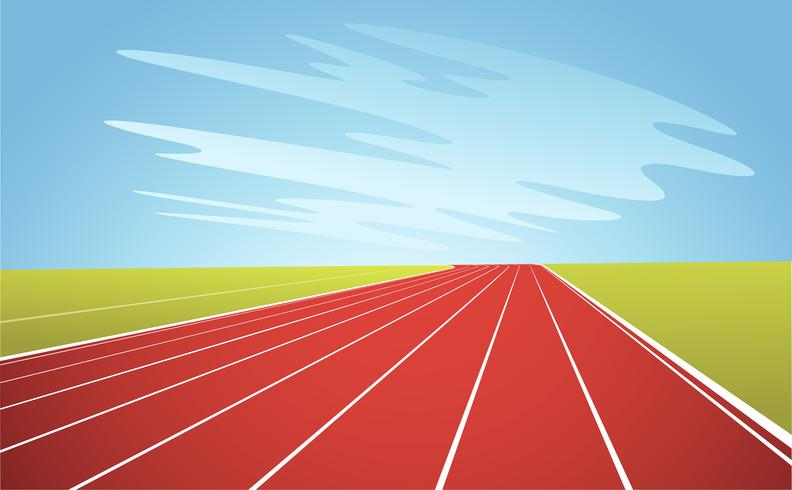
\includegraphics[width=1\textwidth]{pista}
                \caption{Drone Carcará}
                \roundpic[xshift=0cm,yshift=0cm]{5cm}{5cm}{CARCARA1}
                %\caption{Pista de corrida \cite{agostini2007}}
            \end{figure}
            %}
        \end{center}
    \end{columns}
    %*----------- notes
    \note[item]{Notes can help you to remember important information. Turn on the notes option.}
\end{frame}
%-
%*----------- SLIDE -------------------------------------------------------------
\begin{frame}[t]{Resolução}
  \transdissolve[duration=0.5]

  \begin{itemize}
    \Large
    \item Criação de um drone para o laboratório
    \begin{itemize}
      \large
      \item Maior customização
      \item Certeza da qualidade dos componentes
      \item Expertise
    \end{itemize}

    \item Compra de um drone compatível com ROS
    \begin{itemize}
      \large
      \item Restrição de peças ao fabricante
      \item Praticidade
    \end{itemize}

  \end{itemize}

  %*----------- notes
  \note[item]{Notes can help you to remember important information. Turn on the notes option.}
\end{frame}

%*----------- SLIDE -------------------------------------------------------------
\begin{frame}[t]{Estimativa de orçamento}
    \transboxout[duration=0.5]
    \centering

    \begin{tabular}{ l|c|c|c }
      \textbf{Peça}                & \textbf{Quant.} & \textbf{Valor uni.} & \textbf{Total} \\ \hline
      Helices                      &        4        &      R\$70.00       &   R\$280.00    \\
      Motores Brushless (12V)      &        4        &      R\$120.00      &   R\$480.00    \\
      Controlador ESC              &        4        &      R\$80.00       &   R\$320.00    \\
      Barometro                    &        1        &      R\$100.00      &   R\$100.00    \\
      IMU / MPU                    &        1        &      R\$30.00       &    R\$30.00    \\
      Laser unidirecional          &        1        &      R\$100.00      &   R\$100.00    \\
      Teensy microcontroller       &        1        &      R\$400.00      &   R\$400.00    \\
      Receptor de rádio + Controle &        1        &      R\$620.00      &   R\$620.00    \\
      Adaptador Wi-Fi              &        1        &      R\$100.00      &   R\$100.00    \\
      Estrutura de fibra           &        1        &      R\$350.00      &   R\$350.00    \\
      Bateria de Lipo              &        2        &      R\$250.00      &   R\$500.00    \\
      Power Hub                    &        1        &      R\$100.00      &   R\$100.00    \\ \hline
                                   &                 &                     &   \textbf{R\$3380.00}
    \end{tabular}

    %*----------- notes
    \note[item]{Notes can help you to remember important information. Turn on the notes option.}
\end{frame}
%-
%*----------- SLIDE -------------------------------------------------------------
\begin{frame}[t]{Peças disponíveis}
  \transboxout[duration=0.5]
%  \framesubtitle{Materiais necessarios}
  \centering

  \begin{tabular}{ l | c }
          \textbf{Peça}       & \textbf{Quant.} \\ \hline
    Mint eye (câmera estéreo) & 1               \\
             Câmeras          & 2               \\
        Sensor Ultrassom      & 5               \\
           Jetson Nano        & 1
  \end{tabular}

  \vfill

  %*----------- notes
  \note[item]{Notes can help you to remember important information. Turn on the notes option.}
\end{frame}


\begin{frame}[t]{Drones comerciais}
  \transdissolve[duration=0.5]
  \begin{columns}[t]
    \column{.5\linewidth}
    \begin{figure}
      \caption{Parrot Ardrone 2.0}
      \label{fig:pista}
      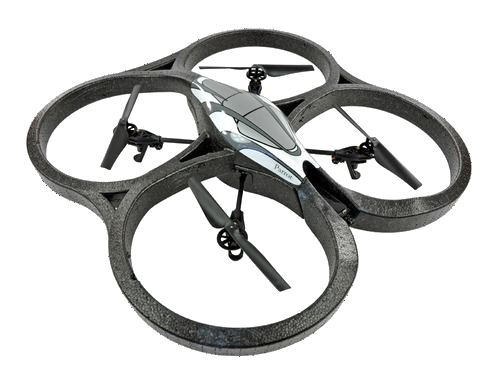
\includegraphics[width=6cm]{Source/pictures/ardrone.png}
    \end{figure}
    \column{.5\linewidth}
    \begin{figure}
      \caption{COEX Clover drone}
      \label{fig:pi2sta}
      \includegraphics[width=6cm]{Source/pictures/COEX-quadcopter.png}
    \end{figure}
  \end{columns}
  %*----------- notes
  \note[item]{Notes can help you to remember important information. Turn on the notes option.}
\end{frame}


\begin{frame}[t]{Drones comerciais}
  \transdissolve[duration=0.5]

  \centering
  \begin{tabular}{ l|c|c|c }
    \textbf{Peça}                & \textbf{Quant.} & \textbf{Valor uni.} &   \textbf{Total}    \\ \hline
    Helices                      &        4        &      R\$70.00       &      R\$280.00      \\
                                 &        4        &      R\$70.00       &      R\$280.00      \\
    Motores Brushless (12V)      &        4        &      R\$120.00      &      R\$480.00      \\
    Controlador ESC              &        4        &      R\$80.00       &      R\$320.00      \\
    Barometro                    &        1        &      R\$100.00      &      R\$100.00      \\
    IMU / MPU                    &        1        &      R\$30.00       &      R\$30.00       \\
    Laser unidirecional          &        1        &      R\$100.00      &      R\$100.00      \\
    Teensy microcontroller       &        1        &      R\$400.00      &      R\$400.00      \\
    Receptor de rádio + Controle &        1        &      R\$620.00      &      R\$620.00      \\
    Adaptador Wi-Fi              &        1        &      R\$100.00      &      R\$100.00      \\
    Estrutura de fibra           &        1        &      R\$350.00      &      R\$350.00      \\
    Bateria de Lipo              &        2        &      R\$250.00      &      R\$500.00      \\
    Power Hub                    &        1        &      R\$100.00      &      R\$100.00      \\ \hline
                                 &                 &                     & \textbf{R\$3380.00}
  \end{tabular}

  %*----------- notes
  \note[item]{Notes can help you to remember important information. Turn on the notes option.}
\end{frame}